\documentclass[]{article}
\usepackage{graphicx}
\usepackage{amsmath,amsfonts,amssymb}
\usepackage[font=small,labelfont=bf]{caption} % Required for specifying captions to tables and figures
\graphicspath{ {./Images/} }

%opening
\title{Computer Vision Assignment One @ ETH Zurich \\ \large Calibration}
\author{Ossama Ahmed 18-936-872}

\begin{document}

\maketitle

\section{Introduction}\

A camera is used to project 3D world points onto 2D image plane. Camera calibration is an essential step in many computer vision applications and it can be considered the first step in most of them. Calibration is the process to find the internal camera parameters that is responsible for this projection process. These parameters are:
\begin{enumerate}
\item - Image center
\item - Focal length
\item - Lens distortion parameters
\end{enumerate}
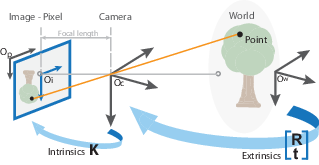
\includegraphics{calibration_overview.png}
\captionof{figure}{Calibration parameters}
\break
In this assignment two widely known calibration algorithms, Direct Linear Transform (DLT) and Gold Standard Algorithm, are implemented in MATLAB and discussed in comparison to using the standard calibration toolbox for MATLAB, Bouget's Calibration Toolbox. 
\newline

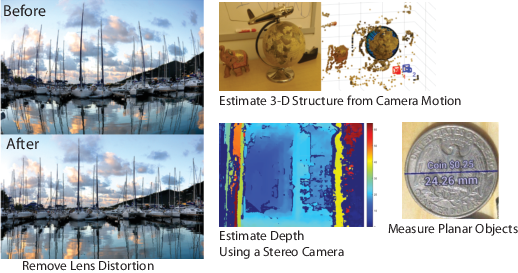
\includegraphics{example.png}
\captionof{figure}{Camera calibration usages}

\section{Data Normalization}\

Data normalization is the first step that was done before implementing the two calibration algorithms mentioned above. Since the points were entered in cartesian coordinates, they were converted to homogenous vectors by just appending 1 in the n+1 dimension. Therefore we ended up with $\mathbf{ x = (x, y, 1)}^\intercal$  and $\mathbf{ X = (x, y, z, 1)}^\intercal$. To transform the points centroid entered manually on the image to the center of the coodinate system, the current centroid was calculated by averaging out all the points coordinates in every direction so that we can shift the points by the mean. 

Secondly, to ensure that the distance from the origin was $\sqrt{2}$ for the image points and $\sqrt{3}$ for the object points, I calculated the current average distance of all points to the origin to caclulate the scale so I can multiply the points with.

After calculating the centroid of the image and object points as well as the scale that will ensure the average distance to the origin is $\sqrt{2}$ and $\sqrt{3}$; the transformation matrices are caculated as the following: \\
$\
U =
\begin{bmatrix}
	xy_{scale}       & 0 &  -xy_{scale}* -xy_{centroid_x}\\
	0     & xy_{scale} & -xy_{scale}* -xy_{centroid_y}\\
	0       & 0 & 1
\end{bmatrix}$

and 

$\
T =
\begin{bmatrix}
xyz_{scale}       & 0  & 0 & -xyz_{scale}* -xyz_{centroid_x}\\
0     & xyz_{scale} & 0 & -xyz_{scale}* -xyz_{centroid_y}\\
0     & 0 &  xyz_{scale}  & -xyz_{scale}* -xyz_{centroid_z}\\
0       & 0 & 0 & 1
\end{bmatrix}$
\section{Direct Linear Transform (DLT)}\
The direct linear transform algorithm is used to minimize the algebric error of the linear system of the camera model. Following the steps specified in the assignment results in the computation of the intrinsic camera matrix K, a rotation matrix R and the camera center C which is then used to calculate the translation matrix since $t = -R*C$. \newline
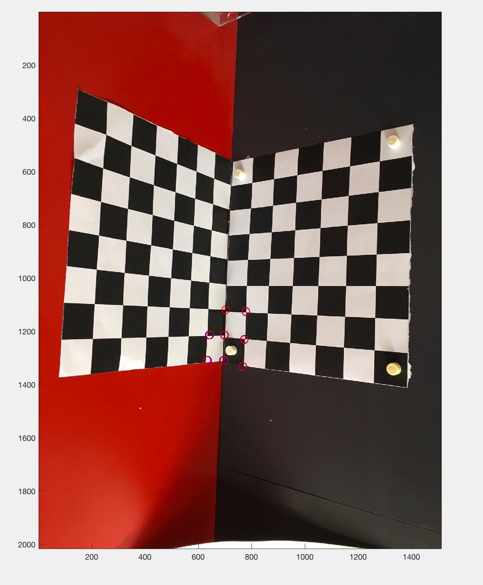
\includegraphics{dlt.png}
\captionof{figure}{Reprojected points of the DLT algorithm; the red points are the original picked ones and the blue points are the reprojected ones}

The following parameters are calculated using the DLT algorithm:

\medskip
$\
K =
\begin{bmatrix}
-814.4       & 6.4  & 504.7\\
0     & 853.8 & 1157.4 \\
0     & 0 &  1
\end{bmatrix}$

\medskip
$\
R =
\begin{bmatrix}
-0.8209       & 0.5658  &   0.0772 \\
0.0709     & -0.0331 & 0.9969 \\
0.5666      & 0.8239 &  -0.0129
\end{bmatrix}$\newline
\newline

\medskip
$\
t =
\begin{bmatrix}
57.0993   \\
-44.2182  \\
-245.8327 
\end{bmatrix}$\newline

\medskip
Finally, I calculated the average error by caclulating the average distance between the reprojected points and the original points. 
$average_{error} = \sqrt{(x_1 - x_2)^2 + (y_1 - y_2)^2} = 0.1088 pixels$\newline

Using the unnormalized points gave a smaller error strangely $average_{error} = 0.1074 pixels$, this might be due to overfitting. Generally speaking using the unnormalized values is numerically unstable for the different operations performed in the DLT algorithms, like SVD for example. Also the negative values in the intrensic matrix K along the diagonal might be because of the choice of the image and the axis drawn on top of it since the lower line is not a straight line like the sample image provided.
\section{Gold Standard Algorithm}\

The gold standard algorithm is used to refine the estimated camera matrix $\hat{p}$ by minimizing the cost function which is the distance between the measured clicked point and the reprojection of the same point.
$cost = \sqrt{(x_1 - x_2)^2 + (y_1 - y_2)^2} $\newline
We use the fminsearch function in MATLAB to optimize for this cost function. 

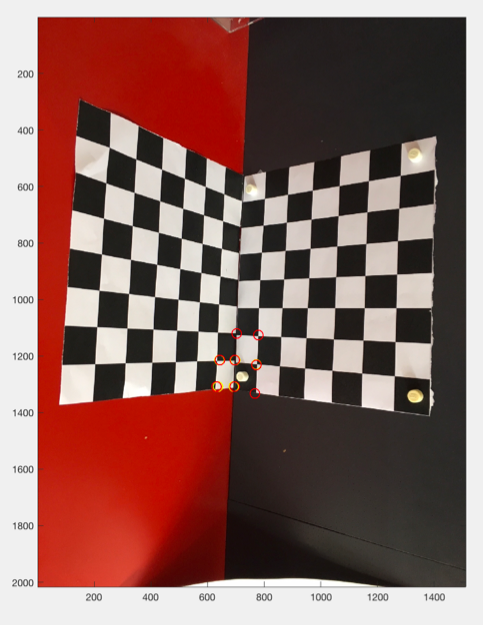
\includegraphics{golden_standard.png}
\captionof{figure}{Reprojected points of the golden standard algorithm; ; the red points are the original picked ones and the yellow points are the reprojected ones}
\medskip

The following parameters are calculated using the Gold standard algorithm:
$\
K =
\begin{bmatrix}
-815.9       & 7.6  & 503.8 \\
0     & 855.6 & 1156.7 \\
0     & 0 &  1
\end{bmatrix}$

$\
R =
\begin{bmatrix}
-0.8211        &  0.5655  &   0.0771\\
0.0712     & -0.0327 & 0.9969 \\
0.5663     & 0.8241 &  -0.0134
\end{bmatrix}$\newline
\newline
$\
t =
\begin{bmatrix}
 57.3254   \\
-44.4194  \\
-246.2886
\end{bmatrix}$\newline
Finally, I calculated the average error by caclulating the average distance between the reprojected points and the original points. 
$average_{error} = \sqrt{(x_1 - x_2)^2 + (y_1 - y_2)^2} = 0.0816 pixels$\newline
\section{Bouget's Calibration Toolbox}\
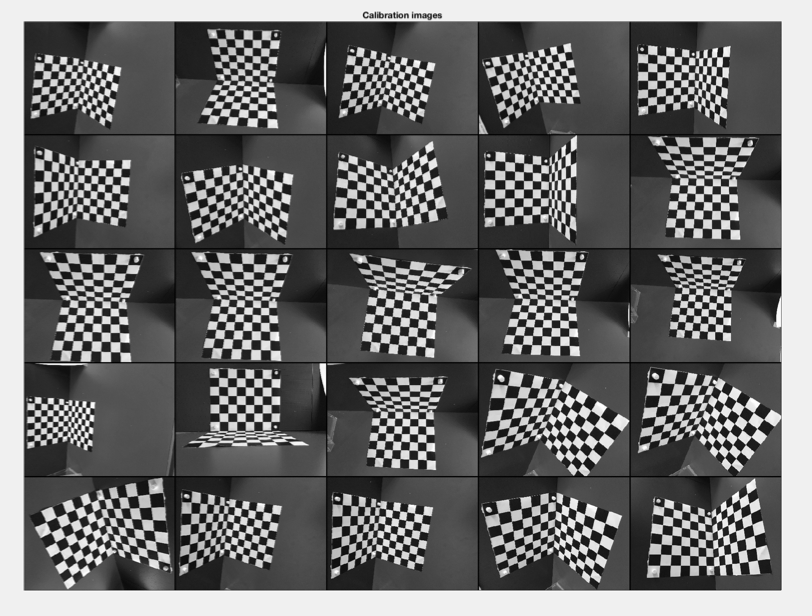
\includegraphics{uncalibrated_images.png}
\captionof{figure}{Input Images}

I used 25 images to follow the tutorial and calibrate the camera, I only used one of the checkerboards printed in the images for calibration and marking the corners; since I had to use the same origin for all the images for proper calibration.

 
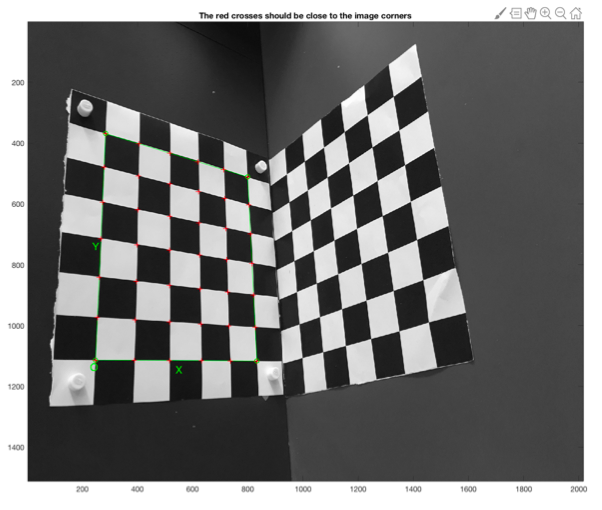
\includegraphics{calibrated_1.png}
\captionof{figure}{Marking corners}

After marking the corners and using the toolbox calibration algorithm, I got the following results: \newline

$\
focallength =
\begin{bmatrix}
1703.086  & 1703.086
\end{bmatrix}$\newline

$\
principlepoint =
\begin{bmatrix}
1007.5  & 755.5
\end{bmatrix}$\newline

$\
skew =
\begin{bmatrix}
0.0
\end{bmatrix}$\newline

$\
distortion =
\begin{bmatrix}
0.0 & 0.0 & 0.0 & 0.0
\end{bmatrix}$\newline

$\
error =
\begin{bmatrix}
0.7523 & 0.9289
\end{bmatrix}$\newline
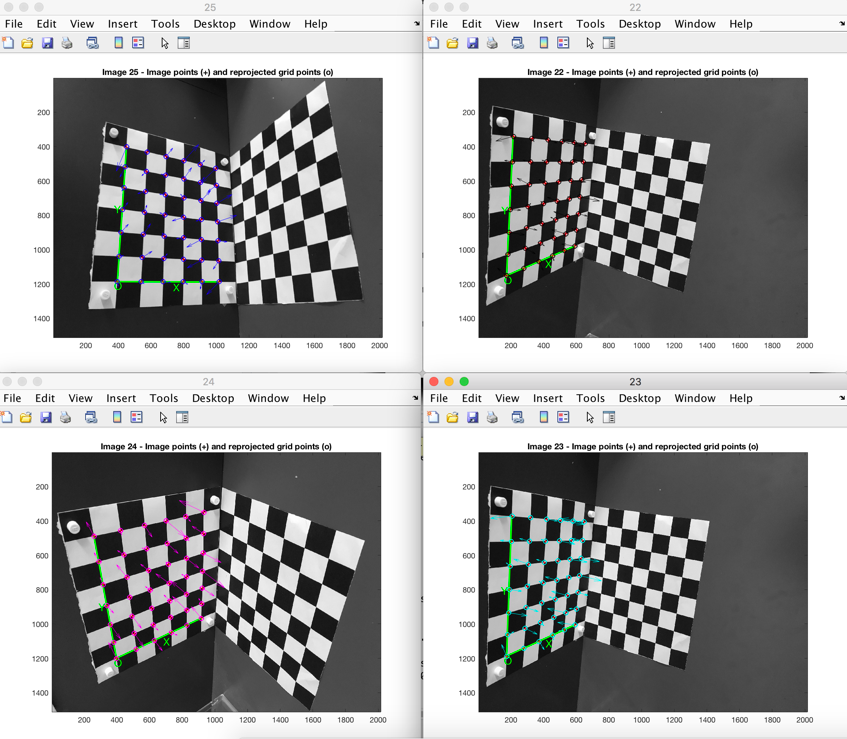
\includegraphics{calibrated_images.png}
\captionof{figure}{After calibration and reprojection}

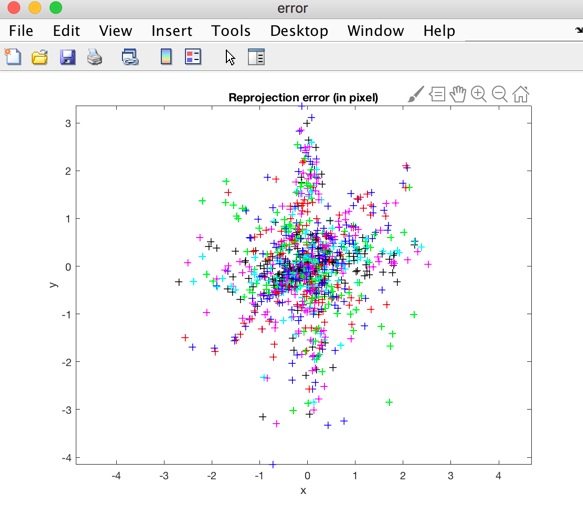
\includegraphics{calibration_error.png}
\captionof{figure}{Calibration error}
\section{Conclusion}\

The error in the gold standard algorithm is much lower than the DLT algorithm error by almost 24\% and using the bouget calibration toolbox was less accurate increasing the error by more than 88\%. One of the reasons is that using the toolbox, there is more data points available compared to just using 6 data points from one image (in the case of the DLT and the Gold Standard ones). Also I found it challenging to manually entering the cartesian coordinates for the image that I chose since the axes drawn on the picture didnt match the checkerboard edges; which resulted in one negative value in the x direction of the intrinsic matrix, given that there is an illusion that part of the checkerboard is behind the camera. 

\end{document}
